\chapter{Camera Geometry}
\label{ch:camera}
In this chapter we provide a basic background about image formation, camera geometry, multiview geometry and OpenGL notation. 
The system proposed in this thesis builds its principles and its implementation on these tools. 
We first, describe how the image projects on a standard camera, by describing the classical pin-hole model and the transformations involved. 
Then we extend the discussion to the two or multiple view case, where more than one camera look at the scene. Multiple camera are needed to reconstruct the 3D structure of a general scene.
Finally, we describe how openGL renders 3D models and we provide a connection with the standard pin-hole model.


\minitoc
\newpage

\section{Image Formation}
The understanding of how the image has been generated is crucial in most computer vision applications. For instance to reconstruct the 3D geometry of the scene, a model that describes how the scene project on the images is needed. 
The classical approach to describe image formation, relies on the so called pin-hole camera model.
This model is a very effective compromise between mathematical simplicity and expressiveness.

Let assume that the world reference frame has its center $C$ in the camera center, the $Z$ axis along the principal axis of the camera, and the $Y$ and $X$ axis oriented upward and left-wise (Figure \ref{fig:pinhole}). 
We define $f$ as the focal length, that is the distance between the camera center and the image plane.
With basic geometry (see Figure \ref{fig:pinhole}(b)), the relation between  point $\mathbf{X} = \{X, Y, Z\}$ and $\mathbf{x}$ can be expressed as follows:
\begin{equation}
\label{eq:proj}
 \mathbf{x} = 
 \begin{pmatrix}
 fX/Z\\
 fY/Z\\
 f
 \end{pmatrix}
\end{equation}
The $x$ and $y$ coordinates of this point represent the position of $\mathbf{x}$ in the image plane, where the 2D reference frame is defined by the axis $x_{\text{cam}}$ and $y_{\text{cam}}$ which lay on the image plane and intersect the principal axis.
By representing $\mathbf{X}$ and $\mathbf{x}$ in homogeneous coordinates, Equation \ref{eq:proj} writes:
\begin{equation}
\label{eq:intrSimple}
 \mathbf{x}^{\text{cam}} = 
 \begin{pmatrix}
 x^{cam}\\
 y^{cam}\\
 1
 \end{pmatrix} =
 \begin{pmatrix}
 fX\\
 fY\\
 Z
 \end{pmatrix}=
 \begin{pmatrix}
 f&0&0&0\\
 0&f&0&0\\
 0&0&1&0
 \end{pmatrix} 
 \begin{pmatrix}
 X\\
 Y\\
 Z\\
 1
 \end{pmatrix}
\end{equation}

\begin{figure}[t]
\centering
 \begin{tabular}{cc}
  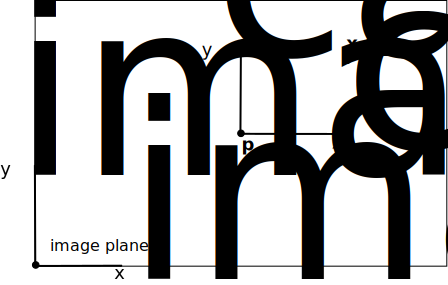
\includegraphics[width=0.45\textwidth]{./img/ch-camera/camera}&
  \includegraphics[width=0.45\textwidth]{./img/ch-camera/camera01}\\
  (a)&(b)
 \end{tabular}
 \caption{Pin-hole camera.}
 \label{fig:pinhole}
\end{figure}
Since an image is represented with a matrix, the coordinates $(0,0)$ are not the center of it; therefore a more practical reference frame on the image plane can be defined as in Figure \ref{fig:centercamera}. Equation \eqref{eq:intrSimple} becomes:
\begin{equation}
\label{eq:intrCompl}
 \mathbf{x}^{\text{image}} = 
 \begin{pmatrix}
 x^{cam} + p_x\\
 y^{cam} + p_y\\
 1
 \end{pmatrix} =
 \begin{pmatrix}
 f&0&p_x&0\\
 0&f&p_y&0\\
 0&0&1&0
 \end{pmatrix} 
 \begin{pmatrix}
 X\\
 Y\\
 Z\\
 1
 \end{pmatrix}
\end{equation}.
The matrix 
\begin{equation}
\label{eq:kmatr}
K = 
\begin{pmatrix}
 f&0&p_x\\
 0&f&p_y\\
 0&0&1
 \end{pmatrix} 
\end{equation}
is named \emph{intrinsic camera} matrix, and $f$, $p_x$ and $p_y$ are the \emph{intrinsic parameters}. 

\begin{figure}[t]
\centering
  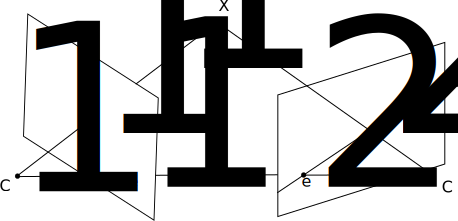
\includegraphics[width=0.9\columnwidth]{./img/ch-camera/camera02}\\
 \caption{Coordinates on the image plane.}
 \label{fig:centercamera}
\end{figure}
The assumption of a world reference frame coinciding with the camera frame is a very particular case. We now generalize the previous relation between a 3D point in the a generic world reference frame $\mathcal{W}$ and the 2D point in the image plane where the 3D point projects.
Let $C^\mathcal{W}$ be the center of the camera in the world reference $\mathcal{W}$ and  $R_\mathcal{C}^\mathcal{W}$ the rotation of the camera frame $\mathcal{C}$ with respect to $\mathcal{W}$: the matrix 
\begin{equation}
E_\mathcal{C}^\mathcal{W} = 
\begin{pmatrix}
R_\mathcal{C}^\mathcal{W} &C^\mathcal{W}\\
\mathbf{0}&1
 \end{pmatrix}   
\end{equation}
 describes the roto-translation of the camera with respect to the world reference frame.

The 3D point in Equation \ref{eq:intrCompl} is in the camera reference frame, but usually 3D points have to be expressed in the world coordinates. Therefore we rewrite the equation:


\begin{equation}
 \mathbf{x}^{\text{image}} =
\begin{pmatrix}
 K &\mathbf{0}
 \end{pmatrix} 
 \mathbf{X}^\mathcal{C}
 = 
\begin{pmatrix}
 K &\mathbf{0}
 \end{pmatrix} 
\begin{pmatrix}
 E_\mathcal{C}^\mathcal{W}
 \end{pmatrix}^{-1}
 \mathbf{X}^\mathcal{W}
\end{equation}
The matrix 
\begin{equation}
  E = (E_\mathcal{C}^\mathcal{W})^{-1} = E_{\mathcal{W}}^{\mathcal{C}} = 
\begin{pmatrix}
R_\mathcal{W}^\mathcal{C} & - R_\mathcal{C}^\mathcal{W} C^\mathcal{W}\\
\mathbf{0}&1
 \end{pmatrix}
\end{equation}
is usually referred as \emph{extrinsic camera} matrix: it is a rototranslation that transforms points in world coordinates to the camera reference frame.

In conclusion, the projection of a 3D point in the world to the image plane is computed as
\begin{equation}
 \mathbf{x}^{\text{image}}
 = 
\begin{pmatrix}
 K &\mathbf{0}
 \end{pmatrix} 
E
\:
 \mathbf{X}^\mathcal{W}\:=
P
\:
 \mathbf{X}^\mathcal{W}
\end{equation}
where matrix $P$ is the \emph{calibration matrix} which express both the parameters intrinsic to the specific camera (intrinsic matrix) and the position and orientation of the camera (extrinsic matrix).


\section{Multi-View Geometry}
In the reconstruction process two or more views are involved, indeed two or more 2D measurements are needed to disambiguate and estimate the 3D position. 
In this section we explain the basic principles underlying the geometry of two cameras in the projective space described thus far.
\subsection{Epipolar geometry}
The geometry between two views is known as \emph{epipolar geometry}: it depends only on the camera parameters, and is independent from the structure of the observed scene.
The epipolar geometry originates whenever two cameras look at the same scene. 
Let $C_1$ and $C_2$ be two cameras defined by the intrinsic matrices $K_1$ and $K_2$ and the extrinsic matrices $E_1$ and $E_2$.
A point $X$,  visible from both cameras, projects in the 2D point $x_1$ and $x_2$ of the $C_1$ and   $C_2$ image plane.
The camera centers $C_1$ and $C_2$, the points $x_1$ and $x_2$ and $X$ lays on the same plane $\pi$ (Figure \ref{fig:epipolar}) named \emph{epipolar plane}. 
If our information about $X$ is represented only by the projection $x_1$, we can deduce that the projection on $C_2$ of the corresponding 3D point is constrained to lay on the line $l_2$, named \emph{epipolar line}, which is the projection of the viewing ray from $C_1$ to $x_1$.



\begin{figure}[t]
\centering
  \includegraphics[width=0.9\columnwidth]{./img/ch-camera/cameraEpipolar}\\
 \caption{Two view: epipolar geometry.}
 \label{fig:epipolar}
\end{figure}
\subsection{The fundamental matrix \texorpdfstring{$F$}{F}}
The epipolar geometry of two views is synthesize into the so called \emph{fundamental matrix}, which represents a projective transformation that maps the point belonging to the image plane of one camera, to the lines of the other camera.

Given two cameras with calibration matrices $P_1$ and $P_2$, we look for the mapping between a point $\mathbf{x_1}$ located in the image plane of the first camera and the corresponding epipolar line $\mathbf{l_2}$. 
The line $\mathbf{l_2}$ is the projection on the image plane of the second camera of the line through the center $C_1$ and the point $\mathbf{x_1}$ in world coordinates, \ie, $P_1^+\mathbf{x_1}$, where $P_1^+$ is the pseudo-inverse of $P_1$ such that $P_1P_1^+ = \mathbf{I}$.
Therefore, $\mathbf{l_2}$ pass through the projection of these two points, \ie, $P_2C_1$ and $P_2P_1^+\mathbf{x_1}$, and is defined as:
\begin{equation}
 \mathbf{l_2} =  P_2C_1 \times P_2P_1^+\mathbf{x_1},
\end{equation}
where $P_2C_1$ is the epipole $e_2$. The fundamental matrix $F$ can be derived as:
\begin{equation}
 \mathbf{l_2} =  \mathbf{e_2} \times P_2P_1^+\mathbf{x_1} = [\mathbf{e_2}]_{\times} (P_2P_1^+)\mathbf{x_1} = F \mathbf{x_1},
\end{equation}
where $[\mathbf{e_2}]_{\times}$ is the skew matrix:
\begin{equation}
  [e]_{\times} =
  \begin{pmatrix}
    0   & -e_3 & e_2\\
    e_3 &   0  & -e_1\\
   -e_2 &  e_1 & 0
  \end{pmatrix}.
\end{equation}
if we know the mapping between 2D points on the two image plane, \eg, we know that $\mathbf{x_1}$ and $\mathbf{x_2}$ are the projection of the same point, the following relation, named \emph{epipolar constraint} is valid:
\begin{equation}
  \mathbf{x_2}^{T} F \mathbf{x_1} = 0.
\end{equation}
Indeed the point  $\mathbf{x_1}$ induces the epipolar line $\mathbf{l_2} = F \mathbf{x_1}$ and the point $\mathbf{x_2}$ lays on this line, \ie, $\mathbf{x_2}^{T} \mathbf{l_2} =  F \mathbf{x_1} = 0$.

\subsection{Triangulation}
In principle, if the epipolar geometry of two cameras is perfectly know, \ie, the fundamental matrix and the 2D point correspondences, the 3D point that generates the two projection is easy to recover as the intersection of the two visibility rays $r_1$ and $r_2$. 
In real cases the 2D projection is affected by noise, therefore the rays are skew and no intersection exists; the 3D position $\mathbf{X}$ needs to be estimated.

\subsubsection{Linear triangulation} 
The \emph{linear triangulation} is the simplest approach to estimate the 3D point $\mathbf{X}$ given the measurements $\mathbf{x_1}$ and $\mathbf{x_2}$ in two cameras whose calibration matrices are $P_1$ and $P_2$.
The combination of the two relations $\mathbf{x_1} = P_1 \mathbf{X}$ and $\mathbf{x_2} = P_2 \mathbf{X}$ leads to a linear system in the form $A\mathbf{X} = \mathbf{0}$. 
For the first camera, we can rewrite the previous relations as:
\begin{equation}
  \mathbf{x_1} \times P_1 \mathbf{X} = \mathbf{0} \rightarrow 
  \begin{cases}
    x_1(\mathbf{p_1}^{3T}\mathbf{X}) -    (\mathbf{p_1}^{1T}\mathbf{X}) = 0\\
    y_1(\mathbf{p_1}^{3T}\mathbf{X}) -    (\mathbf{p_1}^{2T}\mathbf{X}) = 0\\
    x_1(\mathbf{p_1}^{2T}\mathbf{X}) - y_1(\mathbf{p_1}^{1T}\mathbf{X}) = 0
  \end{cases}
\end{equation}
where $P_1 = \begin{smallmatrix}(\mathbf{p_1}^1 \\ \mathbf{p_1}^2\\ \mathbf{p_1}^3)\end{smallmatrix}$ and $P_2 = \begin{smallmatrix}(\mathbf{p_2}^1 \\ \mathbf{p_2}^2\\ \mathbf{p_2}^3)\end{smallmatrix}$.
An analogous relation can be written for the second camera.
The resulting system:
\begin{equation}
  \begin{pmatrix}
    x_1\mathbf{p_1}^{3T} -    \mathbf{p_1}^{1T}\\
    y_1\mathbf{p_1}^{3T} -    \mathbf{p_1}^{2T}\\
    x_1\mathbf{p_1}^{2T} - y_1\mathbf{p_1}^{1T}\\
    x_2\mathbf{p_2}^{3T} -    \mathbf{p_2}^{1T}\\
    y_2\mathbf{p_2}^{3T} -    \mathbf{p_2}^{2T}\\
    x_2\mathbf{p_2}^{2T} - y_2\mathbf{p_2}^{1T}
  \end{pmatrix}
  \mathbf{X} = \mathbf{0}
\end{equation}
is linear and can be solved by SVD decomposition.

\subsubsection{Optimal method to minimize the geometric error}
The previous method results in the minimization of an algebraic error, while a more accurate estimation can be achieved by minimizing the geometric error, \ie, by minimizing the error directly on the domain where lays the noisy measurements.
Let $\mathbf{x_1}$ and $\mathbf{x_2}$ be two noisy measurements of the point $\mathbf{X}$ in two cameras: the noise implies that they usually do not satisfy the epipolar constraint. In order to estimate $\mathbf{X}$ we ideally look for the two points $\hat{\mathbf{x_1}}$ and $\hat{\mathbf{x_2}}$, projection of the estimate $\hat{\mathbf{X}}$ that satisfy $\hat{\mathbf{x_2}}^{T} F \hat{\mathbf{x_1}} = 0$ and  minimize the function:
\begin{equation}
\label{eq:errReproj}
  d(\mathbf{x_1}, \hat{\mathbf{x_1}})^2 + d(\mathbf{x_2}, \hat{\mathbf{x_2}})^2
\end{equation}
where $d(\cdot,\cdot)$ is the Euclidean distance. 

To find the optimal solution that minimize the reprojection error \eqref{eq:errReproj}, we need to rewrite it conveniently as a function of a single variable.

First, let notice that the constraint $\hat{\mathbf{x_2}}^{T} F \hat{\mathbf{x_1}} = 0$ implies that the point $\hat{\mathbf{x_2}}$ lies on the epipolar line $l_1$, and $\hat{\mathbf{x_1}}$ lies on the epipolar line $l_2$. We can write \eqref{eq:errReproj} as:
\begin{equation}
\label{eq:errReproj2}
  d(\mathbf{x_1}, \mathbf{l_1})^2 + d(\mathbf{x_2}, \mathbf{l_2})^2.
\end{equation}
We parametrize line $\mathbf{l_1}(t)$ by $t$  and we compute the corresponding epipolar line $\mathbf{l_2}(t)$ through the fundamental matrix $F$. Equation \eqref{eq:errReproj2} now becomes:
\begin{equation}
\label{eq:errReproj3}
d(\mathbf{x_1}, \mathbf{l_1}(t))^2 + d(\mathbf{x_2}, \mathbf{l_2}(t))^2,
\end{equation}
which is a function of a single variable $t$. 
The minimization problem can now be solved by finding the root of polynomial function \eqref{eq:errReproj3}.

\subsection{Gauss-Newton for Position Refinement}
In case of multiple cameras that see the same point $\mathbf{X}$, we want to take into account all the noisy measurements of the 3D point in order to achieve a more accurate and robust estimate of it.
Equation \eqref{eq:errReproj} for $N$ cameras becomes:
\begin{equation}
\label{eq:errReprojmulti}
\sum_i=1^N d(\mathbf{x_i}, \hat{\mathbf{x_i}})^2,
\end{equation}
where $\mathbf{x_i}$ is the measurements of the point $\mathbf{X}$ in the $i$-th camera and $\hat{\mathbf{x_i}}$ is the reprojection of $\mathbf{X}$ on the same camera $i$. By making the projection explicit:
\begin{equation}
 \label{eq:errReprojmulti2}
\mathcal{C}(\mathbf{X}) =\sum_i=1^N d(\mathbf{x_i}, P_i\mathbf{X})^2 = \sum_i=1^N ||\mathbf{x_i} - proj_i(\mathbf{X})||^2,
\end{equation}
where $proj_i(\mathbf{X}) = P_i\mathbf{X}$ is the projection function for the $i$-th camera .
Therefore, the optimal method described in the previous paragraph can not be applied.
Classical methods to optimize $\mathcal{C}$ and estimate the 3D position of $\mathbf{X}$ are the gradient descent, the Gauss-Newton and the Levenberg-Marquardt algorithms. 
They are iterative methods bootstrapping from an initial guess $\mathbf{X}_0$; at the $k$-th iteration the estimate of the parameter $\mathbf{X}$ can be written as:
\begin{equation}
  \label{eq:minim}
 \mathbf{X}_k = \mathbf{X}_{k-1} + \Delta_{k-1}.
\end{equation}
The three methods differs on how they compute the value of the update $\Delta_{k-1}$.

In the gradient descent, the update follows the decreasing direction of the function computed as the inverse of the gradient evaluated at the current value of $\mathbf{X}$:
\begin{equation}
  \label{eq:discGrad}
 \Delta_{k-1} = - \gamma \nabla {proj}(\mathbf{X}_{k-1}).
\end{equation}
where $\gamma$ is a weighting coefficient.

The Gauss-Newton method computes the decreasing direction by approximating the function with the Taylor expansion; the update becomes:
\begin{equation}
  \label{eq:gaussN1}
    \Delta_{k-1}  = \mathbf{J}_{\mathcal{C}}^{-1} \mathcal{C}(\mathbf{X}_{k-1}) = - (\mathbf{J}_{proj}^T \mathbf{J}_{proj})^{-1} \mathbf{J}_{proj}^T\mathcal{C}(\mathbf{X}_{k-1}),
\end{equation}
where $\mathbf{J}_{\mathcal{C}}=\frac{\partial \mathcal{C}}{\partial \mathbf{X}}$ is the Jacobian of $\mathcal{C}$ and $\mathbf{J}_{proj}=\frac{\partial proj}{\partial \mathbf{X}}$ is the Jacopian of the reprojection function $proj$.

Finally, the Levenberg-Marquardt method combines the two previous with a coefficient $\lambda$, also known as \emph{damping factor}:
\begin{equation}
  \label{eq:l-m}
 \Delta_{k-1} = - (\mathbf{J}_{proj}^T\mathbf{J}_{proj} - \lambda diag(\mathbf{J}_{proj}^T \mathbf{J}_{proj}))^{-1}\mathbf{J}_{proj}^T \mathcal{C}(\mathbf{X}_{k-1}).
\end{equation}
The dumping factor is usually changed for each iteration in order to act similarly to gradient descent in the neighborhood of the minimum, and similarly to Gauss-Newton when we are far from the minimum \cite{Lo05}.culo

The Jacobian $\mathbf{J}_{proj}$ is:
\begin{multline}
  \mathbf{J}_{proj}=\frac{\partial proj}{\partial \mathbf{X}} = \\ =
  \begin{pmatrix}
   \frac{p_{0,0}^i \cdot z - p_{2,0}^i \cdot x}{z^2} & \frac{p_{0,1}^i \cdot z - p_{2,1}^i \cdot x}{z^2} & \frac{p_{0,2}^i \cdot z - p_{2,2}^i \cdot x}{z^2}\\
   \frac{p_{1,0}^i \cdot z - p_{2,0}^i \cdot y}{z^2} & \frac{p_{1,1}^i \cdot z - p_{2,1}^i \cdot y}{z^2} & \frac{p_{1,2}^i \cdot z - p_{2,2}^i \cdot y}{z^2}\\
  \end{pmatrix}
\end{multline}
with $(x,y,z)^T = P_i \mathbf{X}$.


\section{The OpenGL Camera model}
The camera model an the relations described thus far is usually referred to as HZ (Hartley-Zisserman) from the authors of the masterpiece of computer vision \cite{hazi04} that described and adopted this model extensively.
Other disciplines, such as computer graphics, adopt different conventions to describe the scene and the cameras. 
Since we developed the photometric refinement described in Chapter \ref{ch:incrDenseRef} with OpenGL \cite{opengl}, in this paragraph we describe the differences with respect to the HZ model and we derive the convenient transformations to switch from one representation to the other.

\subsection{The OpenGL rendering pipeline}
OpenGL is a rendering and computational engine that processes a 3D mesh. 
Each 3D vertex of the mesh is rendered on the screen after a sequence of transformations. In Figure \ref{fig:camtrans} we represent the transformations involved in both the OpenGL (top) and the HZ (bottom) models.

First, the 3D coordinates of a vertex are transformed from the model to the world reference frame through the model matrix. 
In computer graphics is often useful to decouple the model and the world frames in order to have the possibility to move one mesh object, without changing the camera position. 
In our case, the model of the scene is static, therefore, in the following we can overlook this matrix by assuming it as an identity.
The View matrix has a very similar meaning as the extrinsic matrix of the HZ model: it represents the roto-translation from the world to the camera. This transformations let the vertex coordinates to be expressed in the so called eye coordinates, which almost corresponds to the camera coordinates of the HZ model.

Then, a vertex is subject to the perspective and the Normalized Device Coordinates transformations.
OpenGL defines the concept of frustrum which is the portion of the scene that a camera sees (see Figure \ref{fig:perspective}(a)).
To define the extension of the frustrum, OpenGL requires the definition of the image plane position and dimension, by specifying the top, bottom, left and right coordinates and two clipping planes, orthogonal to the $z$ axis, which define the nearest and the farthest points that can be rendered, \ie, which clips the space. 
In Figure \ref{fig:frustrumTop} we show the top view of the frustrum: the darker area represents what the camera sees and what is rendered on the screen. 
The perspective projection maps the point inside the frustrum to a parallelepiped. 
Then, the NDC matrix together with the division by the fourth component w scale the parallelepiped into a cube such that each point inside it has coordinates $(x,y,z,w)$ :
\begin{equation}
 x \in [-1,1], \:
 y \in [-1,1], \:
 z \in [-1,1] .
\end{equation}

Finally, the cube is scaled and projected on the screen in order to fit the viewport dimension, \ie, the dimension of the displayed image.

\begin{figure}[t]
\centering
 \begin{tabular}{c}
  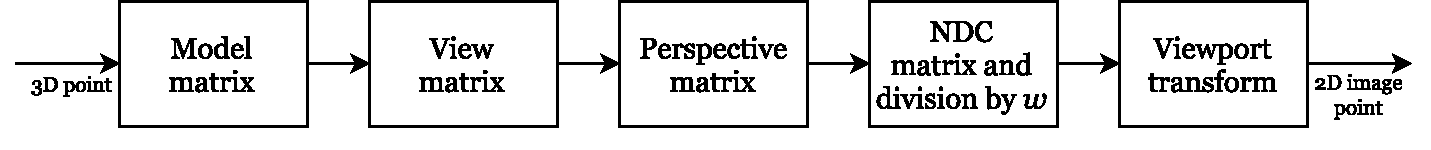
\includegraphics[height=0.1\columnwidth]{./img/ch-camera/cameraopengl-hz01}\\
  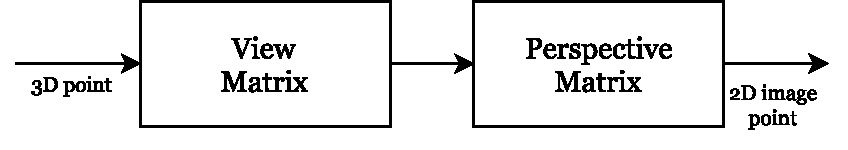
\includegraphics[height=0.1\columnwidth]{./img/ch-camera/cameraopengl-hz02}
 \end{tabular}
 \caption{OpenGL (top) and HZ (bottom) camera transformations.}
 \label{fig:camtrans}
\end{figure}

\begin{figure}[t]
\centering
 \begin{tabular}{cc}
  \includegraphics[width=0.45\columnwidth]{./img/ch-camera/openglcam01}&
  \includegraphics[width=0.45\columnwidth]{./img/ch-camera/openglcam02}
 \end{tabular}
 \caption{OpenGL frustrum before (left) and after (right) the perspective and NDC transformations.}
 \label{fig:perspective}
\end{figure}

\begin{figure}[t]
\centering
 \begin{tabular}{c}
  \includegraphics[width=0.78\columnwidth]{./img/ch-camera/openglcam03}
 \end{tabular}
 \caption{Top view of the OpenGL frustrum.}
 \label{fig:frustrumTop}
\end{figure}
\subsection{From Camera Calibration to OpenGL camera system}
Now we derive the openGL transformation matrices assuming the camera calibration matrix $P = K * E$ is known: let assume we have a 3D point $X = (x,y,z,w)^T$ in homogeneous coordinates, which represents a vertex of the mesh that we need to rendered on the screen with OpenGL, and we aim at simulating the camera projection performed by $P$.

First, as stated in the previous section, we let the Model matrix to be the identity, since we model a static scene rather than objects moving in the world.
\begin{equation}
  model = \mathbf{I}_{4\times4}.
\end{equation}

Then, the View matrix can be derived from the extrinsics matrix:
\begin{equation}
  view = E^{-1}=
  \begin{pmatrix}
    R & \mathbf{t}\\
    \mathbf{0}&1
  \end{pmatrix}^{-1} =
  \begin{pmatrix}
    R^T & -R^T\mathbf{t}\\
    \mathbf{0}&1
  \end{pmatrix}.
\end{equation}

The point $X$ in camera coordinates now becomes:
\begin{equation}
 X^{cam} = model \cdot view \cdot X.
\end{equation}



Once we know the intrinsics parameter of the camera, \ie,  $f_x$, $f_y$, $c_x$ and $c_y$, the perspective projection of OpenGL is very similar to $K$ in Equation \eqref{eq:kmatr}:
\begin{equation}
 persp =
 \begin{pmatrix}
  f_x & 0   & -c_x    & 0\\
  0   & f_y & -c_y    & 0\\
  0   & 0   & (n+f) & n\cdot f\\
  0   & 0   & -1      & 0\\
 \end{pmatrix}
\end{equation}
where the negative sign of the third column acts to flip the z axis according to the openGL convention, which is opposite with respect to the HZ camera; then, the third row is needed to keep the ordering of the depth and to keep the transformed point between the two clipping planes.
The point after the perspective transformation is
\begin{equation}
 X^{orto} = persp \cdot X^{cam}.
\end{equation}

Now we need to scale the scene to a cube with coordinates in the interval  $[-1,1]$ and we remove the points outside the the frustrum. This process is named clipping.

To scale all the coordinates we apply matrix:
\begin{equation}
 NDC =
 \begin{pmatrix}
  \frac{2}{r-l}   &             0   & 0               & -\frac{r+l}{r-l}\\
  0               & \frac{2}{t-b}  & 0               & -\frac{t+b}{t-b}\\
  0               & 0               & -\frac{2}{f-n}  & -\frac{f+n}{f-n}\\
  0               & 0               & 0               & 1\\
 \end{pmatrix}.
\end{equation}
After the last transformation:
\begin{equation}
 X^{clip} = 
 \begin{pmatrix}
  x^{clip}\\
  y^{clip}\\
  z^{clip}\\
  w^{clip}\\
 \end{pmatrix}
 = NDC \cdot X^{orto} = NDC \cdot persp \cdot view \cdot model \dot X
\end{equation}
a point is rendered  only if:
\begin{equation}
 \begin{cases}
  -w^{clip} \leq x^{clip} \leq w^{clip}\\
  -w^{clip} \leq y^{clip} \leq w^{clip}\\
  -w^{clip} \leq z^{clip} \leq w^{clip}\\
 \end{cases}
\end{equation}
and then normalized in the Normalized Device Coordinates system:

\begin{equation}
 X^{NDC} = 
 \begin{pmatrix}
  \frac{x^{NDC}}{w^{NDC}}\\
  \frac{y^{NDC}}{w^{NDC}}\\
  \frac{z^{NDC}}{w^{NDC}}\\
 \end{pmatrix}
\end{equation}


Finally, OpenGL engine renders and adapts the x and y coordinates to the window, which in our case has the image dimensions.








